%! Author = J. Villing
%! Date = 24.07.21

% Preamble
\documentclass[final]{fhnwreport}
% Packages
\usepackage{amsmath}
\usepackage{lipsum}
\usepackage[german]{babel}
\usepackage[style=ieee,urldate=comp,backend=biber]{biblatex}
\usepackage{listings}
\usepackage{pdflscape}
\usepackage{xcolor}
\usepackage{dirtree}
\usepackage{textcomp}
\usepackage{tabularx}
\usepackage{blindtext}
\usepackage{import}
\addbibresource{main.bib}
\graphicspath{{./images/}}

% Custom JS Listing support
\definecolor{mygreen}{rgb}{0,0.6,0}
\definecolor{mygray}{rgb}{0.5,0.5,0.5}
\definecolor{mymauve}{rgb}{0.58,0,0.82}
%Customize a bit the look
\lstset{ %
    backgroundcolor=\color{white}, % choose the background color; you must add \usepackage{color} or \usepackage{xcolor}
    basicstyle=\footnotesize, % the size of the fonts that are used for the code
    breakatwhitespace=false, % sets if automatic breaks should only happen at whitespace
    breaklines=true, % sets automatic line breaking
    captionpos=b, % sets the caption-position to bottom
    commentstyle=\color{mygreen}, % comment style
    deletekeywords={...}, % if you want to delete keywords from the given language
    escapeinside={\%*}{*)}, % if you want to add LaTeX within your code
    extendedchars=true, % lets you use non-ASCII characters; for 8-bits encodings only, does not work with UTF-8
    frame=single, % adds a frame around the code
    keepspaces=true, % keeps spaces in text, useful for keeping indentation of code (possibly needs columns=flexible)
    keywordstyle=\color{blue}, % keyword style
% language=Octave, % the language of the code
    morekeywords={*,...}, % if you want to add more keywords to the set
    numbers=left, % where to put the line-numbers; possible values are (none, left, right)
    numbersep=5pt, % how far the line-numbers are from the code
    numberstyle=\tiny\color{mygray}, % the style that is used for the line-numbers
    rulecolor=\color{black}, % if not set, the frame-color may be changed on line-breaks within not-black text (e.g. comments (green here))
    showspaces=false, % show spaces everywhere adding particular underscores; it overrides 'showstringspaces'
    showstringspaces=false, % underline spaces within strings only
    showtabs=false, % show tabs within strings adding particular underscores
    stepnumber=1, % the step between two line-numbers. If it's 1, each line will be numbered
    stringstyle=\color{mymauve}, % string literal style
    tabsize=2, % sets default tabsize to 2 spaces
    title=\lstname % show the filename of files included with \lstinputlisting; also try caption instead of title
}
%END of listing package%

\definecolor{darkgray}{rgb}{.4,.4,.4}
\definecolor{purple}{rgb}{0.65, 0.12, 0.82}

%define Javascript language
\lstdefinelanguage{JavaScript}{
    keywords={typeof, new, true, false, catch, function, return, null, catch, switch, const, let, var, if, in, while, do, else, case, break},
    keywordstyle=\color{blue}\bfseries,
    ndkeywords={class, export, boolean, throw, implements, import, this},
    ndkeywordstyle=\color{darkgray}\bfseries,
    identifierstyle=\color{black},
    sensitive=false,
    comment=[l]{//},
    morecomment=[s]{/*}{*/},
    commentstyle=\color{purple}\ttfamily,
    stringstyle=\color{red}\ttfamily,
    morestring=[b]',
    morestring=[b]"
}

\lstset{
    language=JavaScript,
    extendedchars=true,
    basicstyle=\footnotesize\ttfamily,
    showstringspaces=false,
    showspaces=false,
    numbers=left,
    numberstyle=\footnotesize,
    numbersep=9pt,
    tabsize=2,
    breaklines=true,
    showtabs=false,
    captionpos=b
}



\title{Google Docs Light}  %Project Title
\author{Workshop Web - FS22}                      %Document Type => Technical Report, ...

\begin{document}
    \maketitle

    \vspace*{\fill}

    \begin{center}
        \renewcommand\arraystretch{2}
        \begin{tabular}{l l}
            Studenten & P. Schmucki, J. Villing, K. Zellweger\\
            Dozenten & D. König, S. Meichtry, J. Luthiger \\
            Studiengang & Informatik\\
            Hochschule & Hochschule für Technik
        \end{tabular}
    \end{center}

    \clearpage

%%---TABLE OF CONTENTS-------------------------------------------------------------------
    \setcounter{tocdepth}{2}
    \tableofcontents
    \clearpage

%%---TEXT--------------------------------------------------------------------------------
    \pagenumbering{arabic}
    \section{Technologie Stack}

Eine zentrale Anforderung an das System ist die konsistente und verzögerungsfreie Darstellung eines Dokuments auf mehreren Klienten.
Die Wahl eines geeigneten Kommunikationsprotokolls ist die Grundlage für eine erfolgreiche Lösung.

Wir verwenden HTTP-Event Streams als Grundlage für die Kommunikation zwischen dem Backend Server und den Klienten.
Als konkrete Implementation dieser Technologie setzen wir Spring-WebFlux ein.
Die weitere Technologieauswahl orientiert sich an diesem Grundsatz Entscheid.

\subsection{Backend Server}
Spring WebFlux ist integriert in das Spring Boot Ökosystem und benötigt daher eine zugrundeliegende JVM\@.
Sprachen die auf der JVM aufbauen, haben den Vorteil, dass sie System Interoperabel sind.

Anstatt Java setzen wir jedoch auf Kotlin als Backend Sprache.
Bis jetzt hat kein Mitglied des Projektteams nennenswerte Erfahrung mit Kotlin und wir möchten diese Gelegenheit nutzen,
die Sprache in einem Projekt näher kennenzulernen.
Wir erwarten die nachfolgenden Vorteile: 

\begin{itemize}
    \item Robuste Implementierung dank Null Safety
    \item Weniger Boilerplate und damit übersichtlichere Implementeirung
    \item Effiziente und Übersichtliche Anwendung von Streams
    \item Schlanke Entitäten und Domänenklassen durch Data Classes
\end{itemize}


\subsection{Frontend Clients}
Kein Teammitglied hat bis jetzt vertiefte Erfahrung im Bereich der Frontend-Entwicklung.
Daher setzen wir auf das an der FHNW vermittelte Framework React, um die Clients zu implementieren.
React bietet mit seinem Komponenten-Model eine einfache Abstraktionsmöglichkeit um die Anwendung sauber zu Kapseln.
Die Funktionalen JSX Komponenten scheinen leichtgewichtiger im Vergleich zu den HTML-Template-Ansätzen von Angular oder VueJS\@.

Unser Ziel ist es in diesem Projekt die Kenntnisse in einem Projekt zu vertiefen und die Client-Software möglichst pur funktional zu halten.


\subsection{Datenbank System}
Um die kollaborativ erstellten Dokumente zu persistieren und zu verwalten setzen wir auf eine No-SQL Lösung.
Das notwendige Datenmodel lässt sich elegant als \emph{Document} abbilden.
Durch den Einsatz einer No-SQL Lösung kann die Representation der Dokumente über alle Layer der Applikation gleichbleibend beibehalten werden,
ohne die Notwendigkeit von ORM\@.

Konkret wird im Projekt MongoDB als Datenbanksystem verwendet.
Wir haben uns für diese Variante aufgrund der bestehenden reaktiven Integration in das Springframework entschieden.


\begin{figure}
    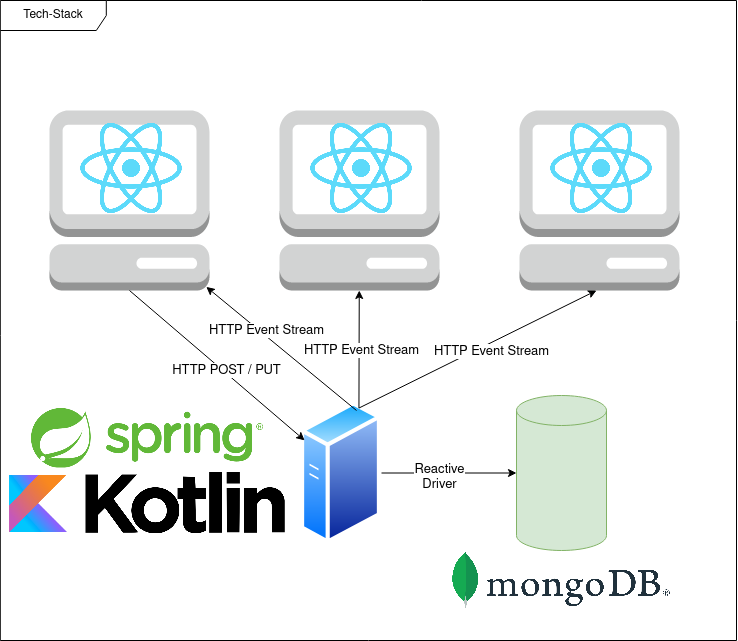
\includegraphics[width=\textwidth,height=\textheight,keepaspectratio]{TechStack}
    \caption{Technologie Stack}
\end{figure}

    \section{Component Model}



\subsection{Frontend}
Das Frontend wird gemäss gängigen Konventionen organisiert.
Komponenten werden zusammen mit ihrem Styling in Ordnern organisiert, Configurationen befinden sich auf top-level und Tests sind abgesondert von normalem Code.

Fast alle Komponenten nutzen den Dispatcher oder einen bestimmten State, um einzelne Commands abzusetzen und den Application State im Redux Store zu manipulieren.

\subsection{Backend}
Zur Organisation der Backend Sourcen orientieren wir uns an der Onion-Architecture.
Die Umsetzung wird aufgrund der geringen Projektgrösse jedoch nicht in unabhängigen Modulen realisiert, sondern über die Package Struktur angedeutet.
Bei der Implementation wird dennoch konsequent darauf geachtet, die einzelnen Layer so zu halten das diese als eigenständige Module extrahiert werden können.

Die erwarteten Layer sind:
\begin{itemize}
    \item Core
    \subitem Model der Dokumente
    \subitem Business Logik zur Konsistenz garantie
    \subitem Command Engine
    \item Service
    \subitem Schnittstelle zwischen Persistenz und API zum Core
    \item Persistence
    \subitem Anbindung an das Datenbanksystem
    \item API
    \subitem Controller für eingehende Dokument Updates
    \subitem Controller für die Reaktive-Streams zu den aktiven Clients.
\end{itemize}

\begin{figure}
    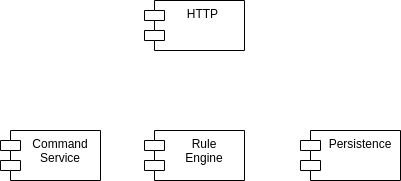
\includegraphics[width=\textwidth,height=\textheight,keepaspectratio]{simple-componentModel}
    \caption{Simple Backend Component Model}
\end{figure}

%%---APPENDIX----------------------------------------------------------------------------

\end{document}
